\chapter{Progettazione}
Prima di poter mettere mano all'applicazione è stato necessario un iniziale periodo di studio dell'ambiente, in particolare del linguaggio \textbf{Dart} e del framework \textbf{Flutter}; è stato piacevole scoprire come Flutter supporti nativamente sia il \textbf{Material Design}, stile adottato per lo sviluppo dell'interfaccia grafica \textit{(almeno per quanto riguarda Android)}, sia lo stile \textbf{Cupertino}, ovvero lo stile nativo di iOS, impostando di default alcune regole di tali stili quando vengono creati determinati widget.

Successivamente a questo periodo di studio è iniziata la vera e propria progettazione dell'applicazione, fase durante la quale sono stati stabiliti il modello dei dati e l'architettura adottata per lo sviluppo. Una nota importante riguardo i dati è che questi sono stati creati da un altro gruppo di persone specializzate in psicologia, che quindi ha ideato, durante lo sviluppo del progetto, le domande necessarie: era dunque necessario che il backend dell'applicazione, qulunque esso fosse stato, permettesse l'accesso sia all'applicazione stessa in lettura che al gruppo di psicologia in scrittura.

\newpage

\section{Glossario}
Prima di procedere e parlare dell'effettiva organizzazione dei dati è necessario e utile definire un glossario di termini ricorrenti utilizzati durante lo sviluppo. Possiamo osservare tale glossario nella Tabella \ref{table:glossario}.

\begin{table}[h!]
\centering
\def\arraystretch{1.5}
\label{table:glossario}
\begin{tabular}{| m{6em} | m{6em} | m{21em} |}
 \hline
 \textbf{TERMINE} & \textbf{SINONIMI} & \textbf{SIGNIFICATO} \\
 \hline \hline
 
 \textbf{Survey} & \textit{Sondaggio, Questionario} & La survey è l'\textit{involucro} più esterno che viene presentato all'utente; contiene uno o più \textit{blocchi}, ognuno dei quali contiene delle domande. Le risposte che vengono inviate sono legate ad essa \textit{(vengono inviate all'endpoint corrispondete al surveyID)}. \\ 
 \hline
 
 \textbf{Block} & \textit{Blocco, \newline Sezione} & Un blocco è una parte di survery, che permette di mostrare le domande in un certo ordine piuttosto che in un altro; se ci sono più blocchi veranno visualizzate prima tutte le domande del primo blocco, e poi quelle del secondo e così via. \\ 
 \hline
 
 \textbf{Question} & \textit{Domanda} & La parte atomica della survey, quella che viene effettivamente legata alla risposta \textit{(tramite il suo ID)}. \\
 \hline
 
 \textbf{Response} & \textit{Risposta} & La risposta vera e propria relativa ad una certa domanda. \\
 \hline
 
 \textbf{Choice} & \textit{Scelta} & Una possibile risposta ad una domanda; se scelta diventa una risposta. \\
 \hline
 
 \textbf{Object} & \textit{Oggetto, Mappa, Map} & Sono gli oggetti JSON presenti nelle risposte alle API. \newline Vengono chiamati anche mappe perché in flutter vengono tradotti in \texttt{Map<key: value>}. \\
 \hline
 
 \textbf{Validation} & \textit{Validazione} & Una serie di regole \textit{(logiche)} che le risposte devono rispettare per essere valide. Il controllo avviene client-side, prima dell'invio. \\
 \hline
\end{tabular}
\caption{Glossario}
\end{table}


\section{Struttura applicazione}
I dati ricevuti prima dell'inizio stesso del progetto riguardavano la struttura dell'applicazione in termini di sezioni e di come queste devono essere organizzate. In particolare, le patologie da identificare e su cui lavorare sono sette: Depressione, Ansia, Pensieri Autodistruttivi, Problemi di Sonno, Burnout, Dolore Cronico e Difficoltà Relazionali. Ognuna di queste problematiche prevede uno specifico \textbf{screening} con una specifica scala che determinerà se l'utente ne è affetto o meno e uno specifico \textbf{percorso terapeutico} della durata di sette settimane. Un'eccezione è fatta per il modulo relativo alle difficoltà relazionali che è \textbf{trasversale} rispetto agli altri: alla sesta settimana tutti gli utenti affronteranno una psico-educazione e degli esercizi relativi alle difficoltà relazionali. Le altre settimane sono caratterizzate da un'iniziale \textbf{psico-educazione} sulle patologie di cui soffre l'utente seguite da una serie di \textbf{esercizi} e da un \textbf{weekly screening} utile per monitorare l'andamento dell'utente. Durante tutto ciò, ogni giorno verrà somministrato all'utente un piccolo questionario giornaliero, notificato ad un orario scelto dall'utente.
Infine, dopo il percorso e dopo 12 e 24 settimane verranno somministrati all'utente gli screening iniziali, in modo da poter avere un'idea del progresso fatto.

È possibile osservare la timeline delle diverse sezioni nella Figura \ref{fig:timeline_app}.

\begin{figure}
\centering
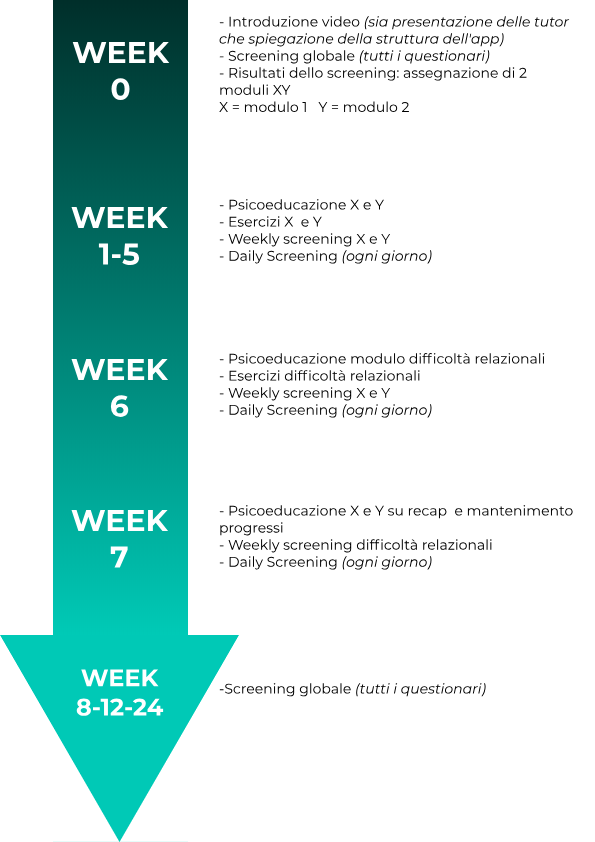
\includegraphics[width=0.8\textwidth]{img/timeline_app}
\caption{Timeline Applicazione}
\label{fig:timeline_app}
\end{figure}

\newpage

In particolare, le diverse sezioni sono:

\renewcommand{\labelitemi}{$\textendash$}
\begin{itemize}
\item \textbf{Introduzione}: la prima cosa presentata all'utente è una introduzione video in cui le tutor di psicologia si presentano e spiegano all'utente cosa affronterà nelle successive settimane.
\item \textbf{Screening}: subito dopo la presentazione iniziale inizia lo screening dell'utente, che consiste in un processo di identificazione e selezione delle patologie di cui \textit{(presumibilmente)} l'utente soffre. Questo processo è realizzato tramite domande mirate che permettano di ottenere un punteggio associato ad ogni patologia secondo diversi algoritmi che dipendono dalla patologia stessa e dalla scala utilizzata per misurarla. Alla fine del processo di screening verranno scelte le due patologie con un punteggio abbastanza alto da essere considerate preoccupanti come patologie su cui lavorare se ce ne sono, altrimenti se solo una patologia ha un punteggio alto verrà scelta, lasciando libera scelta all'utente sulla seconda. Se nessuna patologia ha un punteggio abbastanza alto, l'utente può comunque scegliere due patologie su cui lavorare.
\item \textbf{Esercizi}: una volta identificate le patologie da curare, l'utente affronterà settimanalmente degli esercizi interattivi accompagnati da una lezione di psico-educazione riguardanti le sue patologie; questa è dunque la fase di educazione e di mitigazione dei propri disturbi. Gli esercizi possono essere costituiti da immagini, video e/o audio corredati di qualche domanda sull'argomento in modo da mantenere l'utente concentrato.
\item \textbf{Weekly \& Daily Screenings}: durante il percorso terapeutico vengono somministrati ulteriori screening giornalieri e settimanali sotto forma di domande concise utili a mantenere l'utente concentrato e ad avere un monitoraggio più preciso sul suo progresso.
\end{itemize}

\newpage

\section{Prima di Qualtrics}
Inizialmente non era stato scelto uno specifico backend, per cui lo sviluppo del modello dati è stato eseguito pensando ad un generale database \textit{(come potrebbe essere Firebase)} e ad una generica applicazione che facesse uso di domande e risposte. Come possiamo osservare nella Figura \ref{fig:modello_iniziale}, è stato pensato ad un modello estremamente semplice ma estendibile e che, per il momento, distingueva solo domande a risposta aperta, domande a risposta chiusa e domande \textit{"speciali"} di screening (che inizialmente pensavamo fossero solo a risposta chiusa).
Ad ogni domanda erano poi associate delle opzioni selezionabili \textit{(o definibili nel caso di domande a risposta aperta)} e la risposta ad una certa domanda non era altro che l'opzione \textit{(o le opzioni)} selezionata.

\begin{figure}[h]
\begin{center}
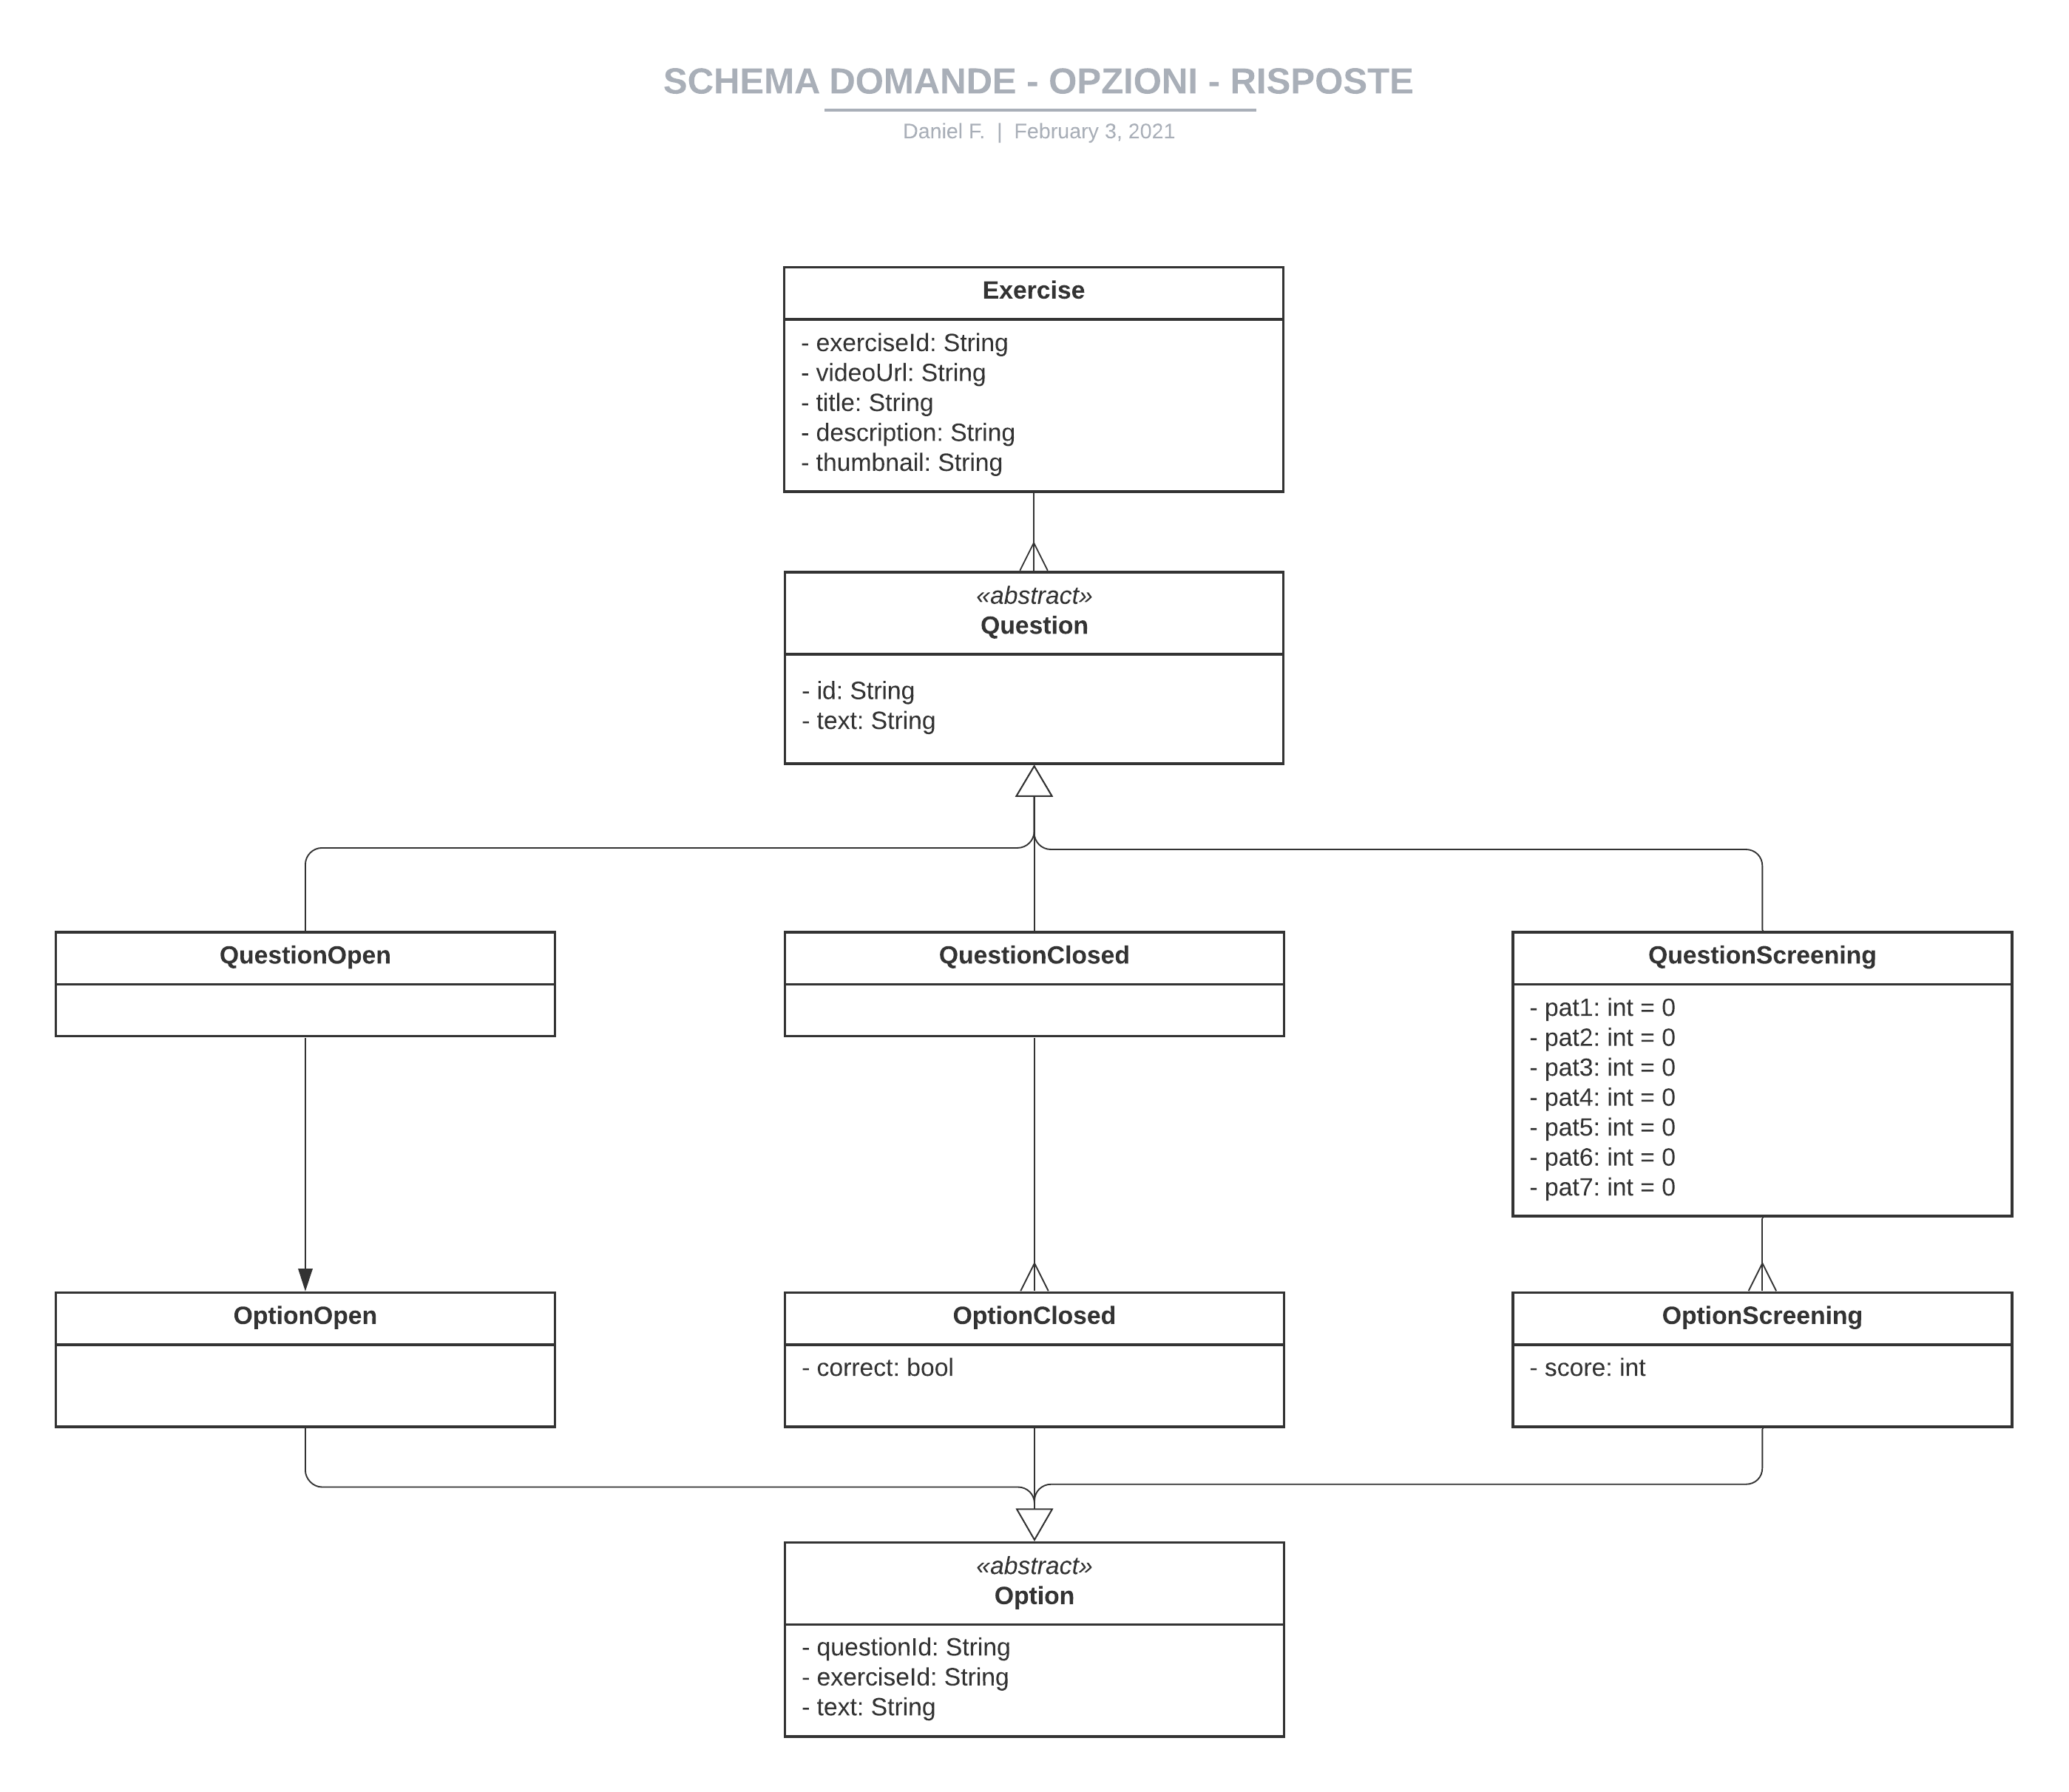
\includegraphics[width=0.95\textwidth]{img/modello_iniziale}
\caption{Modello dati prima di Qualtrics}
\label{fig:modello_iniziale}
\end{center}
\end{figure}


\section{Dopo Qualtrics}
Non molto dopo i primi sviluppi è stato deciso di utilizzare \textbf{Qualtrics}\footnote{\url{www.qualtrics.com/uk/core-xm/survey-software}} come effettivo backend dell'applicazione, che non è altro che una piattaforma per le indagini online che consente di creare sondaggi con vari gradi di complessità che vanno incontro a diverse esigenze di ricerca.
Generalmente questa soluzione è orientata alle aziende per ottenere feedback sia dai propri clienti che dai propri impiegati: l'idea era adattare questo software già pronto e che presenta già diversi tipi di domande utili al nostro scopo per poter ottenere gli input necessari dai nostri utenti e presentarli a chi deve poi analizzarli. Non solo, essendo una piattaforma a sé stante, essa permette anche al gruppo di psicologia di creare i sondaggi necessari indipendentemente dallo sviluppo dell'applicazione, che si limita, tramite le API di Qualtrics, a ottenere e presentare questi sondaggi.

\subsection{Modello dati: domande}
In particolare, come possiamo vedere nel modello semplificato della Figura \ref{fig:modello_semplice_qualtrics}, il modello dati adottato da Qualtrics prevede un oggetto esterno, la \textbf{Survey} \textit{(sondaggio)}, che contiene, oltre a vari parametri di configurazione, una lista di \textbf{Questions} \textit{(domande, che sono degli oggetti anch'esse)} che possono essere di vario tipo; le domande a loro volta contengono i loro parametri di configurazione ed una lista di possibili risposte \textit{(Choices)} se a risposta chiusa.
Tra i valori interessanti contenuti nei parametri delle domande ci sono il \texttt{QuestionText}, che rappresenta la domanda vera e propria in linguaggio naturale, il \texttt{Selector} che permette di avere domande simili ma differenziate per qualche dettaglio \textit{(ad esempio possiamo avere una domanda a risposta chiusa in cui si possono selezionare più risposte piuttosto che solo una)} e il \texttt{ChoiceOrder}, che stabilisce in che ordine devono apparire le possibili risposte, contenute nell'oggetto \texttt{Choices}.
Ogni entità è inoltre opportunamente identificata.

\newpage

\subsection{Modello dati: blocchi}
Un aspetto particolare riguardo l'organizzazione delle domande nell'ambiente Qualtrics è quello legato ai \textbf{Blocks}, che sono degli insiemi di domande presentati separatamente. Questo permette di non sovraccaricare una schermata di domande ma di suddividerle in parti visualizzate indipendentemente.
Come si può vedere sempre nella Figura \ref{fig:modello_semplice_qualtrics}, i blocchi sono degli oggetti contenuti nell'oggetto \texttt{Survey} che dispongono di un \texttt{BlockID} e di una \texttt{Description}, una descrizione testuale utilizzata per dare un'idea del contesto delle domande presenti nel blocco. Inoltre, i blocchi contengono una lista di oggetti \texttt{BlockElements} che, seppur contente oggetti, non contiene le domande vere e proprie, ma solo gli \texttt{QuestionID} delle domande facenti parte del rispettivo blocco; è necessario quindi un incrocio dei dati nell'applicazione per far sì che le domande rispettino l'ordine dei blocchi.

È presente inoltre, sempre nell'oggetto \texttt{Survey}, un ulteriore oggetto \texttt{SurveyFlow} che contiene l'ordine di visualizzazione dei blocchi in una lista contenente i \texttt{BlockID} corrispondenti \textit{(in quanto potrebbero non essere nel giusto ordine all'interno dell'oggetto \texttt{Blocks})}.

\subsection{Modello dati: risposte}
Sempre nella Figura \ref{fig:modello_semplice_qualtrics} possiamo osservare anche come sono fatte le risposte nel backend; in particolare, essendo ogni entità opportunamente identificata direttamente da Qualtrics, le risposte non sono altro che degli oggetti contenenti delle coppie \texttt{\{ID\_Domanda: ID\_Risposta\}} oppure \texttt{\{ID\_Domanda: [ID\_Risposta\_1, ..., ID\_Risposta\_n]\}}, nel caso di domande a risposta chiusa, mentre nel caso di domande a risposta aperta sono del tipo \texttt{\{ID\_Domanda: "Risposta"\}}. Oltre a questo, possono contenere dei meta-dati che diano informazioni ad esempio sul tempo impiegato per rispondere o eventualmente sul browser utilizzato dagli utenti: di questi dati la maggior parte non verranno prodotti dall'applicazione, essendo opzionali \textit{(ricordiamo che Qualtrics è stato pensato per essere implementato in siti web)}.

\begin{figure}
\centering
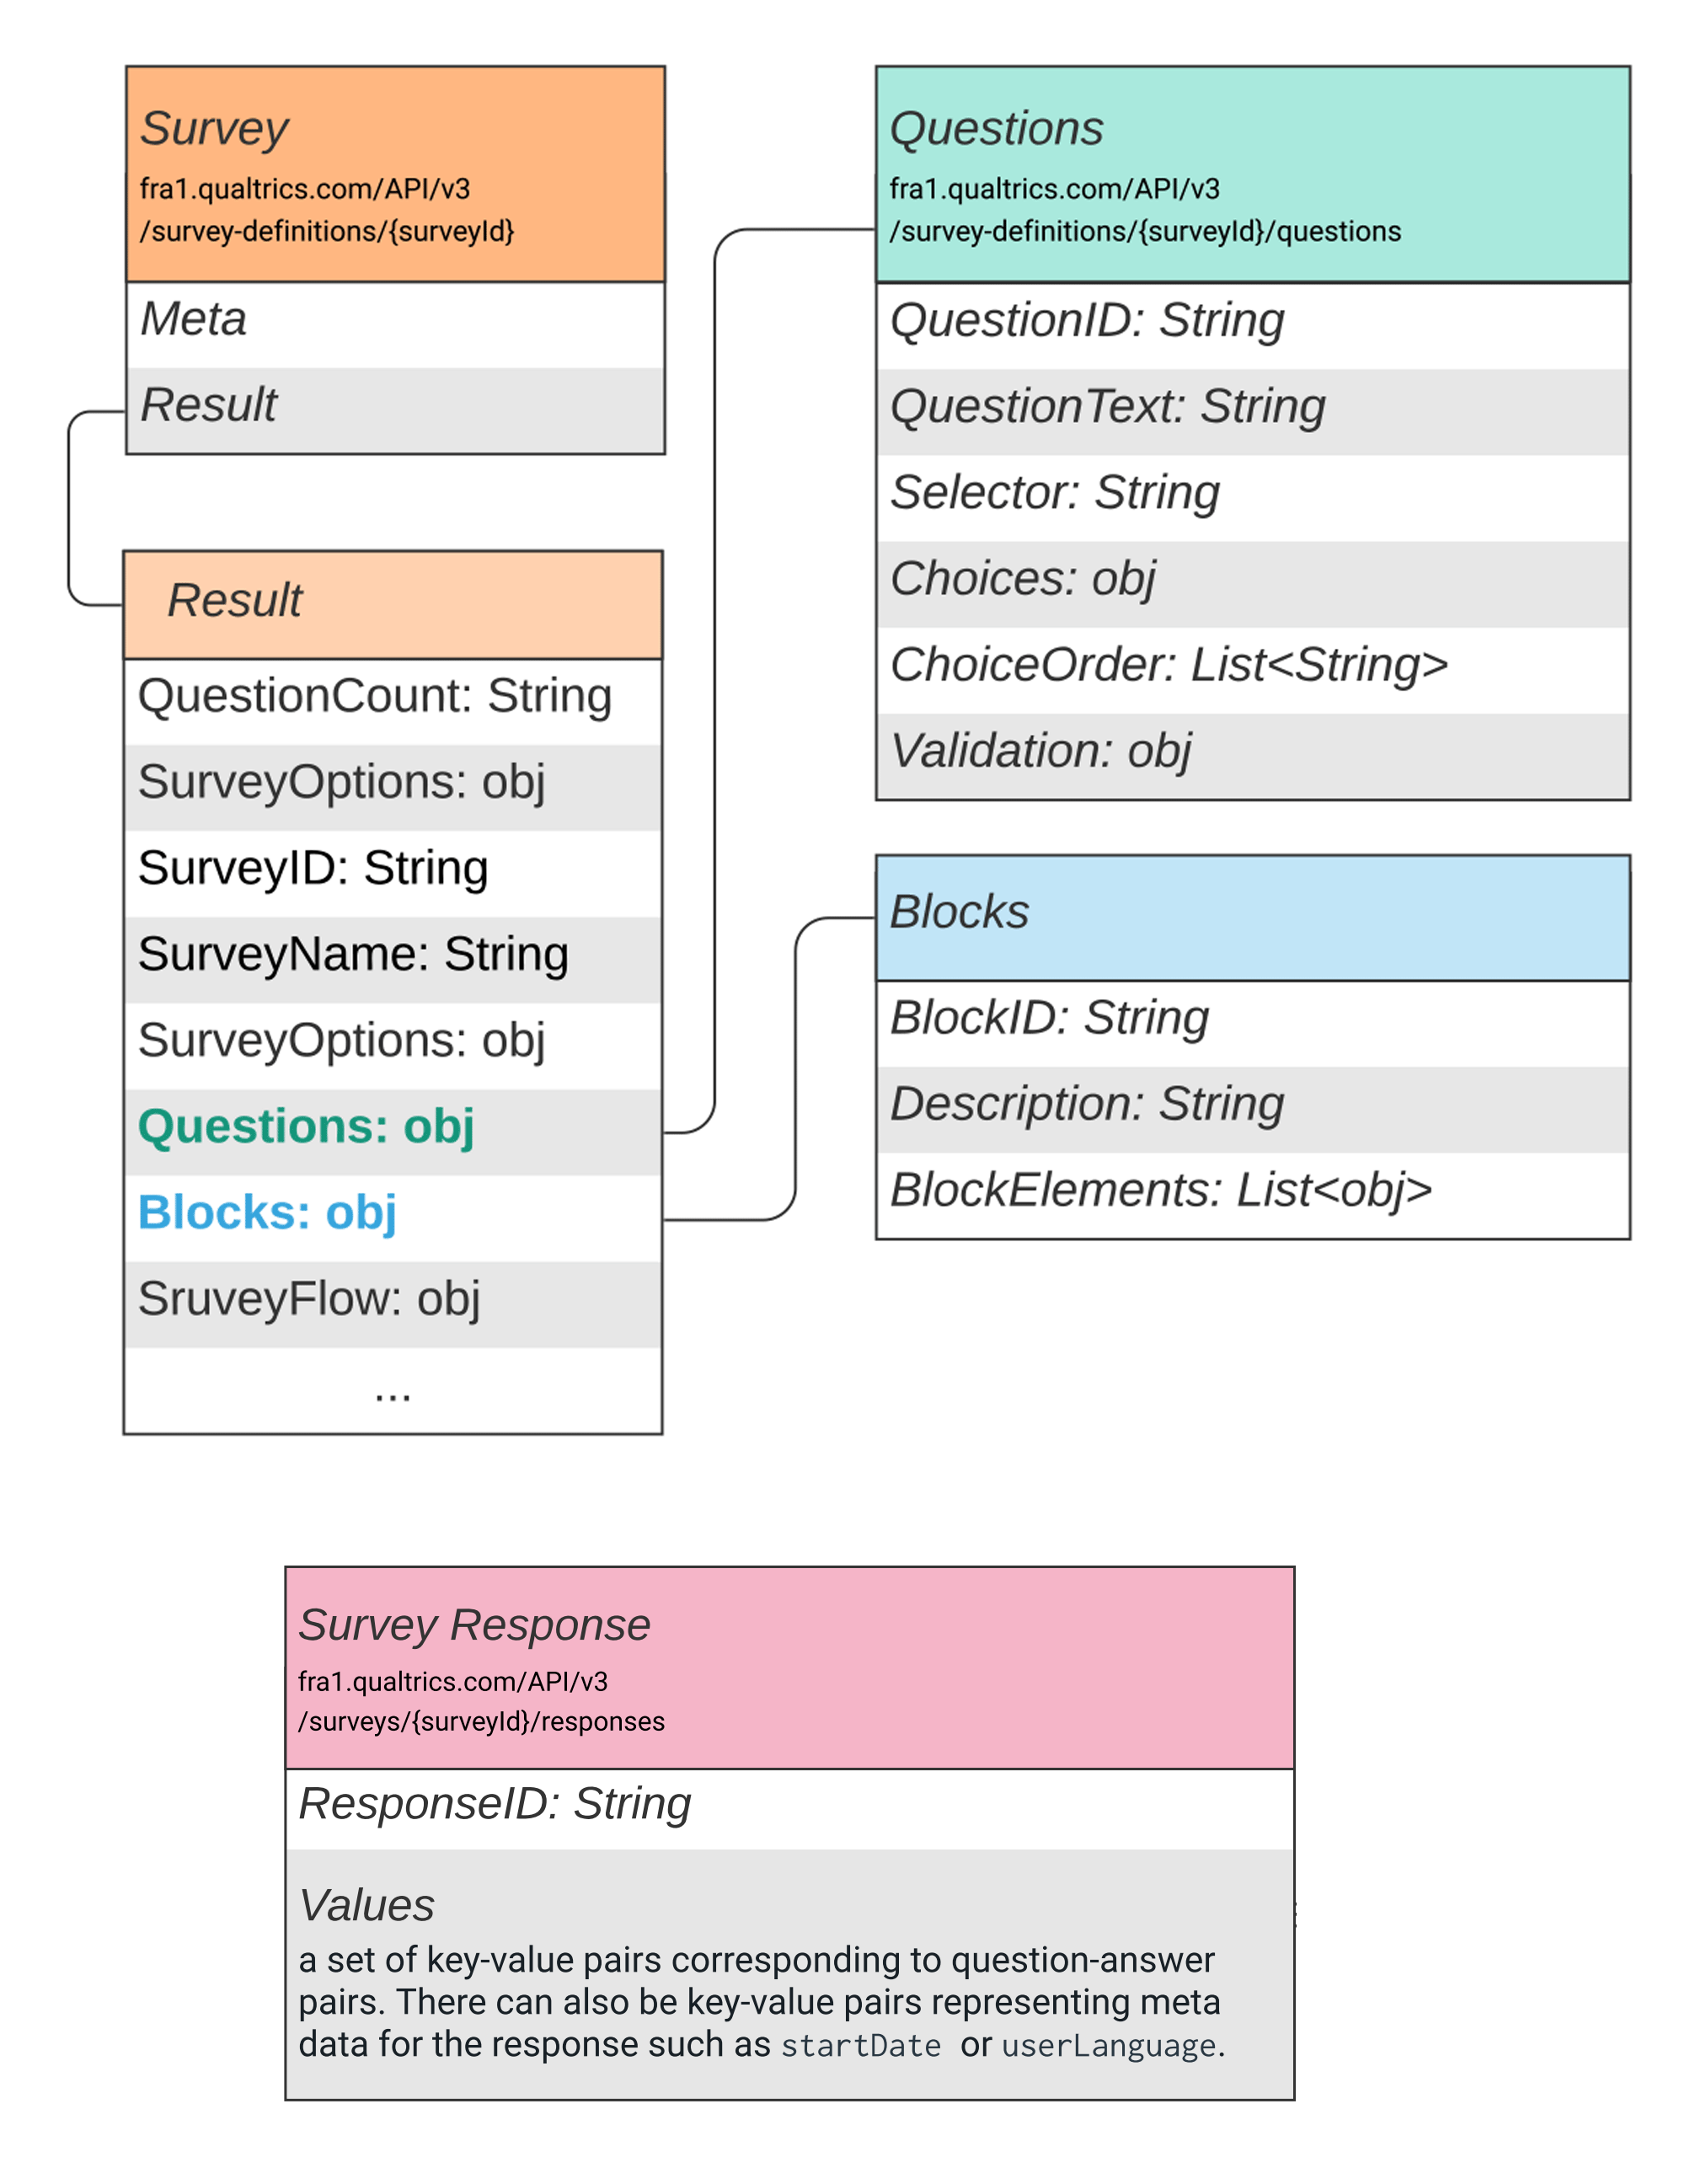
\includegraphics[width=\textwidth]{img/modello_semplice_qualtrics}
\caption{Modello dati Qualtrics semplificato}
\label{fig:modello_semplice_qualtrics}
\end{figure}

\newpage

\section{Architettura adottata}
Per lo sviluppo vero e proprio dell'applicazione è stato adottato il pattern architetturale \textbf{Model-View-Controller \textit{(MVC)}}\cite{MVC}, che è un'architettura che permette di slegare la \textbf{logica di presentazione} dalla \textbf{logica di business} tramite la separazione delle responsabilità tra tre principali componenti software:
\begin{itemize}
\item \textbf{Model}: questo componente fornisce i metodi necessari ad accedere ai dati interni dell'applicazione e aggiorna la \textit{View}.
\item \textbf{View}: i componenti di tipo \textit{View} sono quelli che effettivamente l'utente vede a schermo e con cui interagisce. Questo tipo di componenti espone e presenta i dati all'utente.
\item \textbf{Controller}: i \textit{Controller} sono quei componenti che ricevono effettivamente i comandi dell'utente \textit{(attraverso il View)} e li eseguono modificando lo stato del \textit{Model}.
\end{itemize}

\subsection{MVC in Flutter}
Le componenti \textbf{View} dell'applicazione sono costituite dalla parte atomica di un'applicazione Flutter, gli \textbf{widget}\footnote{\url{https://flutter.dev/docs/development/ui/widgets-intro}}: ogni elemento visibile a schermo è un qualche tipo di widget o una combinazione di widget. Flutter permette di avere degli widget all'interno di altri widget e di definire dei \textbf{custom widget}, costituiti da combinazioni di widget più basilari, per definire delle UI complesse. Man mano che si definiscono diversi widget all'interno dell'applicazione, Flutter crea un \textbf{widget tree}, ovvero un albero che rappresenta la gerarchia tra widget mostrando i vari parent \textit{(widget complessi di livello superiore)} e i children \textit{(widget base definiti da Flutter)} e che verrà poi utilizzato per ottimizzare il rendering dell'UI.
Possiamo osservare un esempio di widget tree nella Figura \ref{fig:widget_tree}.

\begin{figure}[h]
\centering
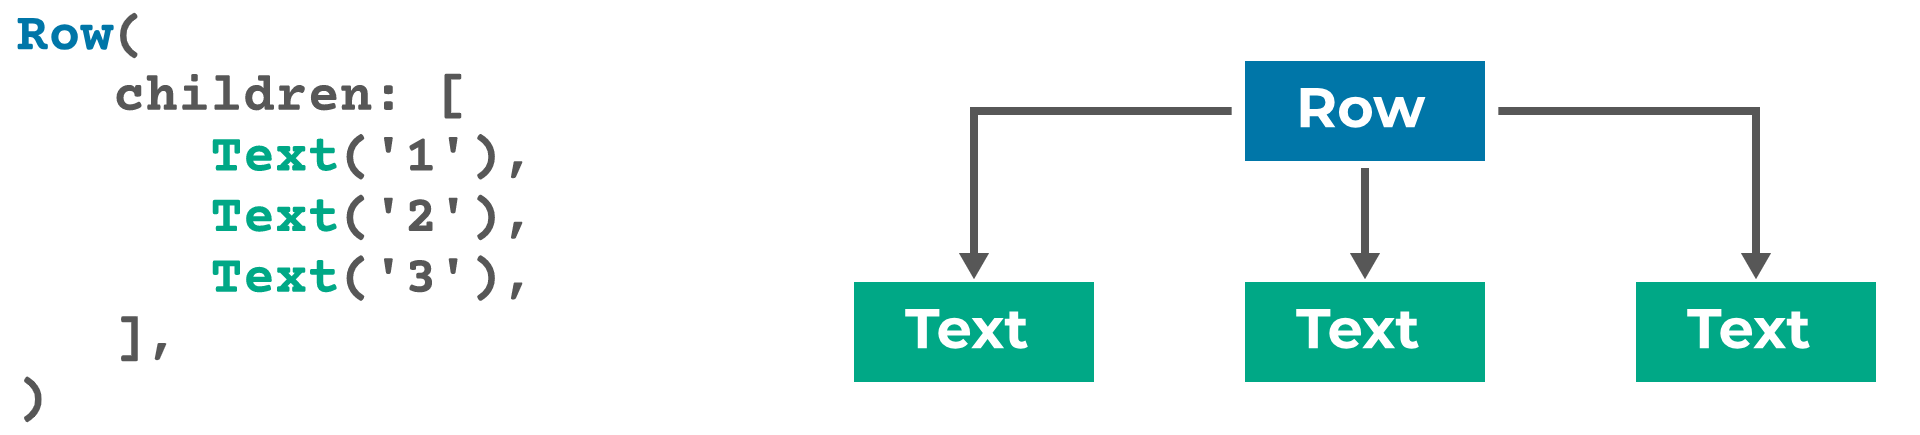
\includegraphics[width=0.6\textwidth]{img/widget_tree}
\caption{Esempio di widget tree}
\label{fig:widget_tree}
\end{figure}

Come è possibile osservare nella Figura \ref{fig:MVC_Flutter}, per realizzare le componenti \textbf{Model} e \textbf{Controller} in Flutter sono stati utilizzati i \textbf{Provider}: un Provider è una classe che viene estesa con la classe \texttt{ChangeNotifier}, che permette alla classe iniziale di ascoltare i cambiamenti nei dati e utilizzarli per aggiornare la \textbf{View} tramite il metodo \texttt{notifyListeners()} \textit{(e che quindi implementa un design pattern di tipo Observer)}. In particolare, i \textbf{Model} sono definiti dalle classi estese con \texttt{ChangeNotifier} che contengono effettivamente i dati e i metodi utilizzabili per modificarli, mentre i \textbf{Controller} sono definiti dall'accesso ai provider nelle classi \textbf{View} tramite la definizione \texttt{Provider.of<Classe>(context)}: questo perché quando viene definito un Provider ad un certo livello del widget tree, tutti gli elementi al di sotto di esso possono accedervi utilizzando il contesto fornito dal framework stesso, evitando così di dover importare ad ogni livello la classe \textbf{Model} per poter accedere ai suoi metodi.

\begin{figure}[h]
\centering
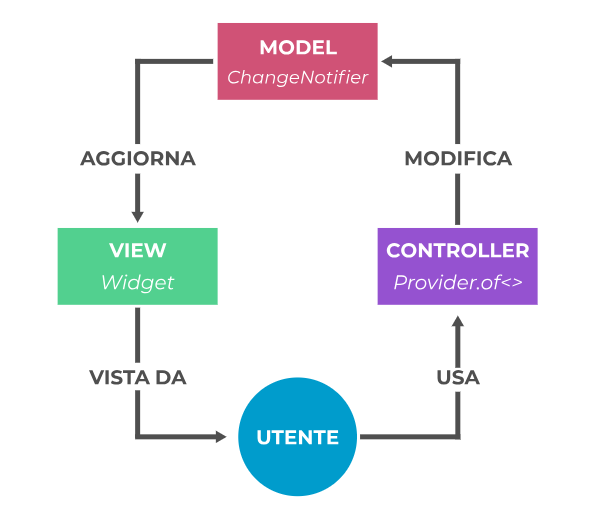
\includegraphics[width=0.8\textwidth]{img/MVC_Flutter}
\caption{Archittetura MVC adottata in Flutter}
\label{fig:MVC_Flutter}
\end{figure}

\section{Interfaccia utente}
Fin da subito è stato condotto uno studio anche su quale sarebbe stato lo stile grafico adottato per l'applicazione: visto il target e l'importanza di un'applicazione del genere è sicuramente molto importante che essa sia facile da utilizzare, intuitiva e gradevole.
Vista la continua crescita e la predisposizione di Flutter verso il \textbf{Material Design}\footnote{\url{https://material.io/}}, si è scelto questo come stile grafico da adottare in quanto fornisce delle linee guida per ottenere semplicità d'uso ed intuitività, lanciando però comunque spazio al designer per rendere il tutto anche visivamente piacevole e personale.

\subsection{Material Design}
Il \textit{Material Design} si è evoluto molto nel tempo nel tentativo di Google di dare agli sviluppatori un sistema di design che aiutasse a creare delle esperienze di alta qualità che siano anche consistenti tra diverse piattaforme come Android, iOS e Web \textit{(ed è anche per questo che Flutter adotta nativamente alcune linee guida di questo stile)} in un ambiente in cui Apple andava molto verso il realismo col suo \textit{scheumorfismo} che però rischiava di distrarre troppo l'utente con i suoi troppi dettagli e dove Microsoft sosteneva il suo \textit{Metro/Flat design} che invece creava confusione su cosa era effettivamente interattivo e cosa no. Google voleva quindi offrire i vantaggi di entrambe le soluzioni utilizzando sia riferimenti al realismo che la semplicità del minimalismo.

\newpage

Difatti, il \textit{Material Design} è molto ispirato al mondo fisico, sopratutto alle sue superfici, al modo in cui esse interagiscono con la luce \textit{(riflettanza, ombreggiatura)} e a come interagiscono fra loro \textit{(due oggetti fisici possono essere impilati, affiancati, ma non potranno mai compenetrarsi)} e cerca quindi di replicare questi comportamenti anche nel mondo digitale: il \textbf{materiale} è come un foglio di carta interattivo.
Dunque, come è possibile notare nella Figura \ref{fig:material_example}, i componenti \textit{Material} interagiscono fra loro come se fossero in un ambiente 3D fatto di sovrapposizioni ed affiancamenti che generano le dovute ombreggiature e riflessi.

\begin{figure}[h]
\centering
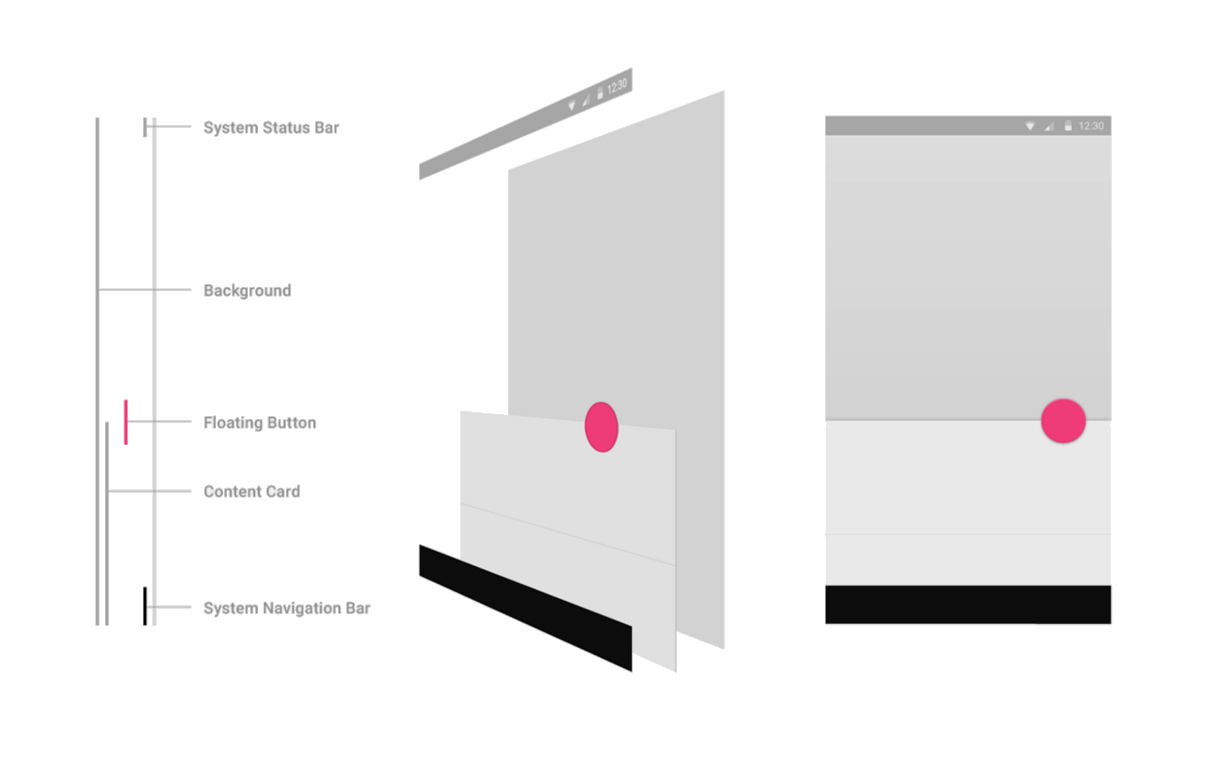
\includegraphics[width=1\textwidth]{img/material_example}
\caption{Esempio di interazione tra diversi componenti Material}
\label{fig:material_example}
\end{figure}


Allo stesso tempo, questo linguaggio visivo implementa anche diversi metodi tradizionali della stampa e della tipografia atti a creare elementi gerarchici con il dovuto focus in modo da attirare l'attenzione dell'utente dove necessario in modo diretto e semplice evitando che quest'ultimo si senta spaesato, utilizzando quindi sempre elementi \textit{flat} metaforizzati però nel mondo reale. È importante sottolineare che queste linee guida permettono di creare un design efficace che sia però comunque originale ed unico alle sensazioni che deve suscitare.